\documentclass[a4paper,11pt,twoside]{article}
\usepackage[utf8]{inputenc}	% Text coding
\usepackage[T1]{fontenc}
\usepackage{lmodern}
\usepackage[czech]{babel}
\usepackage{epsfig}
\usepackage{amsfonts,amsmath,amssymb}
\usepackage{graphicx}
\usepackage[unicode]{hyperref}
%\usepackage{indentfirst}
\usepackage{fancyhdr}
\usepackage{xifthen}
\usepackage{amsthm,thmtools}
\usepackage{bold-extra}
\usepackage[dvipsnames]{xcolor}
\usepackage[subrefformat=simple,labelformat=simple]{subcaption} % Instead of subfigure
\usepackage{listings}
\usepackage{comment}
\usepackage{titlesec}
\usepackage{underscore}
\usepackage{makecell}       % Šířky čar v tabulkách

% Page size
\addtolength{\topmargin}{-1.5cm} %\addtolength{\textheight}{-10cm}
\addtolength{\textwidth}{4cm} \addtolength{\textheight}{4cm} % Width and height of the text
\addtolength{\voffset}{-0.5cm} % Top margin
\addtolength{\hoffset}{-2cm}
\setlength{\headheight}{15pt}

\DeclareMathOperator{\e}{e}

\def\vector#1{\boldsymbol{#1}}								% Vector
\renewcommand{\d}{\mathrm{d}}
\newcommand{\derivative}[3][]{\ifthenelse{\isempty{#1}}	    % Normal derivative
	{\frac{\d{#2}}{\d{#3}}}
	{\frac{\d^{#1}{#2}}{\d{#3}^{#1}}}
}
\newcommand{\im}{\mathrm{i}}

\def\makematrix#1{\begin{pmatrix}#1\end{pmatrix}}       % Matrix
\def\abs#1{\left|#1\right|}
\def\probability#1{\mathrm{Pr}\left[#1\right]}
\def\expectation#1{\mathrm{E}\left[#1\right]}
\def\dispersion#1{\sigma_{#1}^{2}}
\def\c{,\!}

\def\code#1{\textnormal{\texttt{#1}}}
\def\file#1{\textnormal{\textbf{\texttt{#1}}}}
\def\ghfile#1#2{\textnormal{\textbf{\texttt{\href{https://github.com/PavelStransky/PCInPhysics2021/blob/main/#1#2}{#2}}}}}

\def\abbreviation#1{\textnormal{\textsc{#1}}}

\begin{document}

\section*{Domácí úkol na 28.4.2025}
\subsection*{Parciální diferenciální rovnice}
\subsubsection*{Laplaceova rovnice elektrostatického pole}

Uvažujte dva rovnoběžné dráty v rovině (kondenzátor), mezi kterými je elektrické napětí $U=\varphi_{2}-\varphi_{1}$.

\begin{center}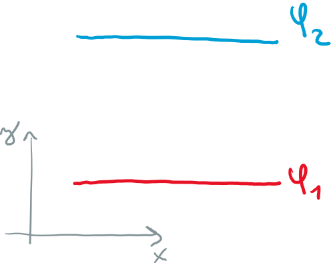
\includegraphics[width=0.25\linewidth]{kondenzator.png}\end{center}

\begin{enumerate}
    \item 
        Vyřešte numericky 2D Laplaceovu rovnici elektrostatického pole
        \begin{equation*}
            \Delta\varphi(x,y)=0
        \end{equation*}
        pro kondenzátor.
        Vykreslete graf potenciálu mezi elektrodami kondenzátoru.

    \item 
        Představte si nyní, že spodní deska kondenzátoru je země a horní deska kondenzátoru je nabitý bouřkový mrak.
        Na zemi stojí osoba (modelujte ji jako vodič), která je navíc vodivě spojená se zemí.
        Její potenciál je tedy roven $\varphi_{1}$.

        \begin{center}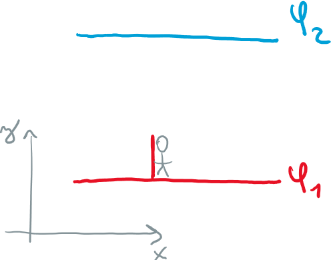
\includegraphics[width=0.25\linewidth]{clovek.png}\end{center}

        Vyřešte Laplaceovu rovnici pro tento případ.

    \item
        Stojící osoba se v potenciálu polarizuje a na jejím povrchu se objeví náboj.
        Pomocí Poissonovy rovnice
        \begin{equation*}
            \Delta\varphi(x,y)=-\frac{\rho(x,y)}{\epsilon_{0}},
        \end{equation*}
        kde $\rho$ je hustota náboje a $\epsilon_{0}$ je permitivita vakua,
        spočítejte hustotu náboje na hlavě člověka.

    \item
        Do blízkosti osoby umístěte \emph{hromosvod}: vodivou tyč vodivě spojenou se zemí, která bude vyšší, než je výška osoby.

        \begin{center}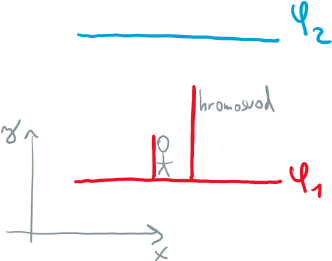
\includegraphics[width=0.25\linewidth]{hromovsvod.png}\end{center}

        Přesvědčte se, že náboj na hlavě osoby se sníží.

    \item
        Vypočítejte a vhodným způsobem zobrazte pro všechny případy intenzitu elektrického pole
        \begin{equation*}
            \vector{E}=-\nabla\varphi(x,y).
        \end{equation*}

    Řešte numericky na mříži o velikosti alespoň $50\times50$ bodů.
    Jednotky, potenciály $\varphi_{1}$ a $\varphi_{2}$, přesnou velikost osoby a hromosvodu a jejich vzdálenost od sebe volte dle vlastního uvážení.

    \end{enumerate}



\end{document}